\chapter{Procesamiento señal de voz}
En este capítulo conoceremos más acerca del procedimiento para procesar la señal de voz, además repasaremos algunos conceptos previos para entender en procesamiento y luego introduciremos 2 conceptos importantes \textit{Extracción de características y la coincidencia de patrones.}

\section{Conceptos previos}
\subsection{Voz}
Los seres humanos diariamente nos comunicamos por medio del habla utilizando nuestras voces somos capaces de transferir información en forma de \textit{ondas sonoras}.\\ Estas ondas transmiten una gran cantidad de información usando el aire como medio de transmisión.
Las propiedades como variaciones en amplitud al empezar o finalizar una palabra varían en el transcurso del tiempo, por lo cual es importante analizar segmentos de tiempo donde estas propiedades se mantengan aisladas de esta manera nos aseguramos que la señal de voz no cambie.
\subsection{Audios}
Los audios son un tipo de \textit{datos no estructurados}, es decir datos que no se encuentran en algún tipo de estructura de datos, estos tipos de datos son los que más se encuentran el mundo real como imágenes y audio. Una características de estos es que son complejos en su recolección y preparación para la realización de un análisis.\\ El audio puede capturarse mediante la grabación de nuestro entorno pero para que este audio sea entendido por las computadoras necesita un formato adecuado como: wav, mp3 y wma. \\
Debido a que el sonido es una señal de onda podemos analizar y obtener valores numéricos de este. En la figura 4.1 observamos una onda de la cual obtenemos valores almacenando las alturas de puntos equidistantes de esta forma guardamos información de esta onda.
\begin{figure}[H]
	\centering
	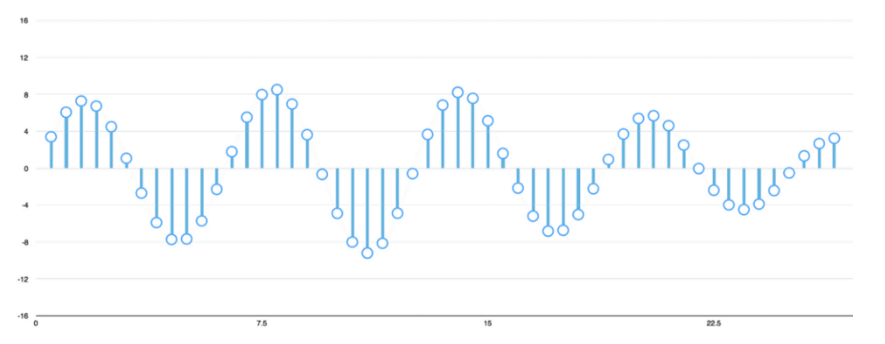
\includegraphics[width=0.9\textwidth]{Figures/onda.png}
	\caption{Onda de sonido \\ Fuente:  \href{https://medium.com/@venkateshpnk22/how-to-convert-your-speech-voice-to-text-data-1b2686099260}{\textit{https://medium.com}}}
	\label{onda}
\end{figure} 
\subsection{Escala mel}
Es una escala psicoacústica propuesta por Stevens, Volkman y Newman 
\begin{figure}[H]
	\centering
	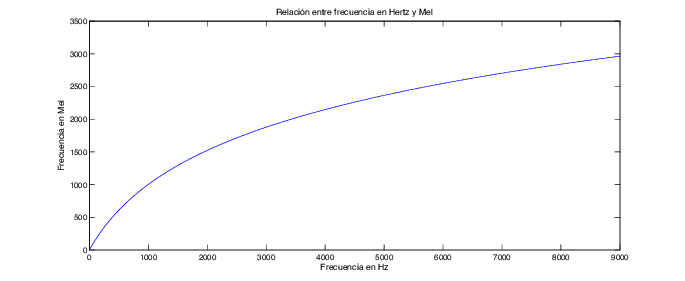
\includegraphics[width=0.9\textwidth]{Figures/escala_mel.png}
	\caption{Relación escala mel - Frecuencia\\ Fuente:  \href{https://www.researchgate.net/figure/Relacion-entre-frecuencia-en-Hz-eje-x-y-en-escala-Mel-eje-y_fig2_312041038}{\textit{https://www.researchgate.net}}}
	\label{mel}
\end{figure} 
\begin{equation}
	\label{STg}
	\begin{aligned}
	m=1127.01048\log_{e}(1+f/700))
	\end{aligned}
\end{equation}
\subsection{Dominio de tiempo}
Este dominio permite obtener la amplitud en un instante de tiempo dado.
\subsection{Dominio de frecuencia}
Este dominio permite representar a nuestra frecuencia de onda como un par de amplitud y valores de la fase. Para señales periódicas se relaciona con series de fourier y para señales no periódicas se relaciona con la transformada de fourier.
\begin{figure}[H]
	\centering
	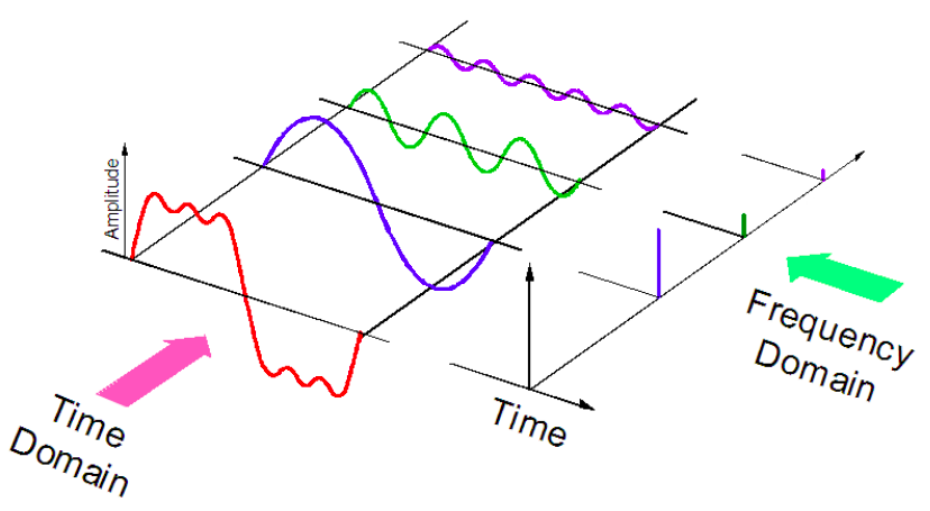
\includegraphics[width=0.9\textwidth]{Figures/audio_signal.png}
	\caption{Dominios de tiempo y frecuencia de dominio\\ Fuente:  \href{https://medium.com/@venkateshpnk22/how-to-convert-your-speech-voice-to-text-data-1b2686099260}{\textit{https://medium.com}}}
	\label{onda}
\end{figure} 


\section{Proceso de extracción de características}

También conocido como análisis de la señal de voz este proceso retené la información necesaria de la voz y elimina los datos redundantes y no necesarios. Este proceso es uno de los más importantes debido a que se transforma la señal en una forma adecuada para los modelos de clasificación. 
\subsection{Etapas del proceso de extracción de carácterísticas}

El proceso de extracción de características puede ser divido en 3 etapas o subprocesos.
\subsubsection{Análisis Espectral}
Cuando un seña de voz es producida esta es variable en el tiempo, por tanto podemos clasificar sus características en función a la actividad espectral.
\begin{itemize}
	\item \textbf{Banco de filtros digitales\\}
	Es un sistema que divide una señal de entrada $x(n)$ en un conjunto de señales $x_{1},x_{2},..$ donde cada una corresponde a una región del espectro de $x(n)$.
	\item \textbf{Transformada de fourier\\}
	\item \textbf{Predicción Lineal\\}
\end{itemize}

\begin{figure}[H]
	\centering
	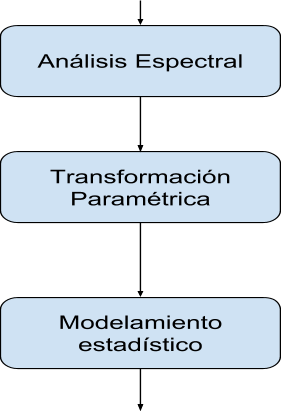
\includegraphics[width=0.4\textwidth]{Figures/proceso.png}
	\caption{Etapas del proceso de extracción de características\\ Fuente:Elaboración propia}
	\label{onda}
\end{figure}

\subsubsection{Transformación de parámetros}
\subsubsection{Modelo estadístico }

\begin{figure}[H]
	\begin{center}
		\begin{tikzpicture}[node distance=2cm]
		\node (input) [startstop] {Capa de Entrada};
		\node (conv1) [startstop, below of=input] {Capa de convolución 1};
		
		\node (pool1) [startstop, below of=conv1] {Capa Pooling 1};
		\node (conv2) [startstop, below of=pool1] {Capa de convolución 2};
		\node (pool2) [startstop, below of=conv2] {Capa Pooling 2};
		\node (full) [startstop, below of=conv2] {Full Layer};
		\node (exit) [startstop, below of=full] {Capa de salida};
		\draw [arrow] (input) -- (conv1) ;
		\draw [arrow] (conv1) -- (pool1);
		\draw [arrow] (pool1) -- (conv2);
		\draw [arrow] (conv2) -- (pool2);
		\draw [arrow] (pool2) -- (full);
		\draw [arrow] (full) -- (exit);
		\end{tikzpicture}
	\end{center}
	\caption{Etapas del proceso \\ Fuente:  \textit{Fuente Propia}}
\end{figure}
\subsection{Algoritmos}
 A continuación describiremos algunos algoritmos que se usan para realizar este proceso.
\subsubsection{Real Cepstral Coefficient(RCC)}
Este algoritmo convierte la señal del dominio de tiempo a dominio de frecuencia aplicando la transformada rápida de fourier a cada cuadro(frame). Luego se aplica le logaritmo y la transforma de fourier inversa. 
\begin{equation}
\label{STs}
\begin{aligned}
Real Cepstrum = IFFT (log (FFT (s (n))))
\end{aligned}
\end{equation}
Donde:
\begin{itemize}
	\item IFFT: Transformada de fourier inversa
	\item FFT: transformada rápida de fourier.
	\item s(n): señal de voz.
\end{itemize}
\subsubsection{Mel Frequency Cepstral Coefficients (MFCC)} 
Es el algoritmo más usado en aplicaciones de reconocimiento de voz, esta basado en el sistema auditivo humano, el cual es sensible a 2 características dinámicas y estáticas. El MFCC se concentra principalmente en las características estáticas. 
\begin{itemize}
	\item Pre-emphasis
	\item Framing
	\item Hamming windowing
	\item Transformada rápida de fourier
	\item Mel filter bank
	\item Discrete Cosine Transform
	\item Delta energy and Delta spectrum
\end{itemize}
\subsubsection{Codificación lineal predictiva} 
Este método también conocido como LCP considera que la señales de voz pueden ser expresadas como la combinación lineal de las anteriores, entonces podemos describir a la señal de voz utilizando los coeficientes de esta combinación lineal. Este método ha sido utilizado para el procesamiento de la señal de voz debido modela el comportamiento del tracto vocal.\\ En el ecuación 4.3 vemos como se expresa la señal de voz $s$ usando las p anteriores señales de voz y los $a_{k}$ representan \textit{coeficientes del LCP.}

\begin{equation}
\label{LPC}
\begin{aligned}
s(n)= \sum_{k=1}^{p}a_{k}s(n-k)+e(n)
\end{aligned}
\end{equation}

\subsubsection{LPCC}

\section{Coincidencia de patrones}

\subsubsection{VQ}
\subsubsection{HMM}
\subsubsection{GMM}
\subsubsection{SVM}
\subsubsection{MLP}
\subsubsection{DTW}